\newsection
\section{Combinatorics}
\subsection{Introduction}
Combinatorics was developed from the willingness of humans to gamble and the fact that everybody wanted to win as much money as possible.

\subsection{Simple counting operations}
The easiest way to find the best chance of winning is to write down all possible outcomes. This can be very tedious though when the list gets longer.

We can note this all down as a list or as a tree diagram. So-called Venn Diagrams might also help represent the relationship between two sets or events. Essentially a Venn Diagram is a graphical representation of set operations such as $A \cup B$.


\subsection{Basic rules of counting}
\subsubsection{Multiplication rule}
If one has $n$ possibilities for a first choice and $m$ possibilities for a second choice, then there are a total of $n \cdot m$ possible combinations.

When we think about a task, and we have an \textbf{and} in between e.g. properties, we need to multiply all the options.

\subsubsection{Addition rule}
If two events are mutually exclusive, the first has $n$ possibilities and the second one has $m$ possibilities, then both events together have $n+m$ possibilities.

When we think about a task, and we have an \textbf{or} in between e.g. properties, then we need to add all the options.


\newpage
\subsection{Factorial}
\begin{definition}[]{Factorial}
    The factorial stands for the product of the first $n$ natural numbers where $n \ge 1$. Notation: $!$
    \[
        n! = n \cdot (n - 1) \cdot (n - 2) \cdot \ldots \cdot 3 \cdot 2 \cdot 1
    \]
    Additionally, $0! = 1$. We read $n!$ as ``\textit{n factorial}''
\end{definition}

\subsubsection{Operations}
We can rewrite $n!$ as $n \cdot (n - 1)!$ or $n \cdot (n - 1) \cdot (n - 2)!$ and so on.

It is also possible to write $7 \cdot 6 \cdot 5$ with factorial notation: $\displaystyle \frac{7!}{4!}$, or in other words, for any excerpt of a factorial sequence: \[n \cdot (n - 1) \cdot \ldots \cdot m = \frac{n!}{(m - 1)!}\]


\subsection{Permutations}
\begin{definition}[]{Permutations}
    A permutation of a group is any possible arrangement of the group's elements in a particular order\\

    \textbf{Permutation rule without repetition:} The number of $n$ \textbf{\textit{distinguishable}} elements is defined as: $n!$
\end{definition}


\subsubsection{Permutation with repetition}
For $n$ elements $n_1,n_2,\ldots,n_k$ of which some are identical, the number of permutations can be calculated as follows:
\[
    p = \frac{n!}{n_1! \cdot n_2! \cdot \ldots \cdot n_k!}
\]
where $n_k$ is the number of times a certain element occurs. 
As a matter of fact, this rule also applies to permutations without repetition, as each element occurs only once, which means the denominator is $1$, hence $\displaystyle \frac{n!}{(1!)^n} = n!$

\inlineex \smallhspace CANADA has $6$ letters, of which $3$ letters are the same. So the word consists of $3$ A's, which can be arranged in $3!$ different ways, a C, N and D, which can be arranged in $1!$ ways each. Therefore, we have:
\[
    \frac{6!}{3!\cdot 1! \cdot 1! \cdot 1!} = \frac{6!}{3!} = 6 \cdot 5 \cdot 4 = 120
\]

Since $1!$ equals $1$, we can always ignore all elements that occur only once, as they won't influence the final result.


\newpage
\subsection{Variations}
\begin{definition}[]{Variations}
    A \textbf{\textit{variation}} is a selection of $k$ elements from a universal set that consists of $n$ \textit{distinguishable} elements.\\

    \textbf{Variation rule without repetition:} The $_n\mbox{P}_k$ function is used to \textit{\textbf{place}} $n$ elements on $k$ places. In a more mathematical definition:
    The number of different variations consisting of $k$ different elements selected from $n$ distinguishable elements can be calculated as follows:

    \[
        \frac{n!}{(n - k)!} = _n\mbox{P}_k
    \]
\end{definition}

\subsubsection{Variations with repetition}
If an element can be selected more than once and the order matters, the number of different variations consisting of $k$ elements selected from $n$ distinguishable elements can be calculated using $n^k$



\subsection{Combinations}
\begin{definition}[]{Combination}
    A combination is a selection of $k$ elements from $n$ elements in total without any regard to order or arrangement.

    \textbf{Combination rule without repetition:} \[
        _n\mbox{C}_k = {n\choose k} = \frac{_n\mbox{P}_k}{k!} = \frac{n!}{(n - k)! \cdot k!}
    \]
\end{definition}

\subsubsection{Combination with repetition}
In general the question to ask for combinations is, in how many ways can I distribute $k$ objects among $n$ elements?
\[
    _{n + k - 1}\mbox{C}_k = {n + k - 1\choose k} = \frac{(n + k - 1)!}{k!(n - 1)!}
\]



\subsection{Binomial Expansion}
\label{sec:binomial-expansion}
Binomial expansion is usually quite hard, but it can be much easier than it first seems. The first term of the expression of $(a + b)^n$ is always $1 a^n b^0$. Using the formula for combination without repetition, we can find the coefficients of each element:

\begin{center}
    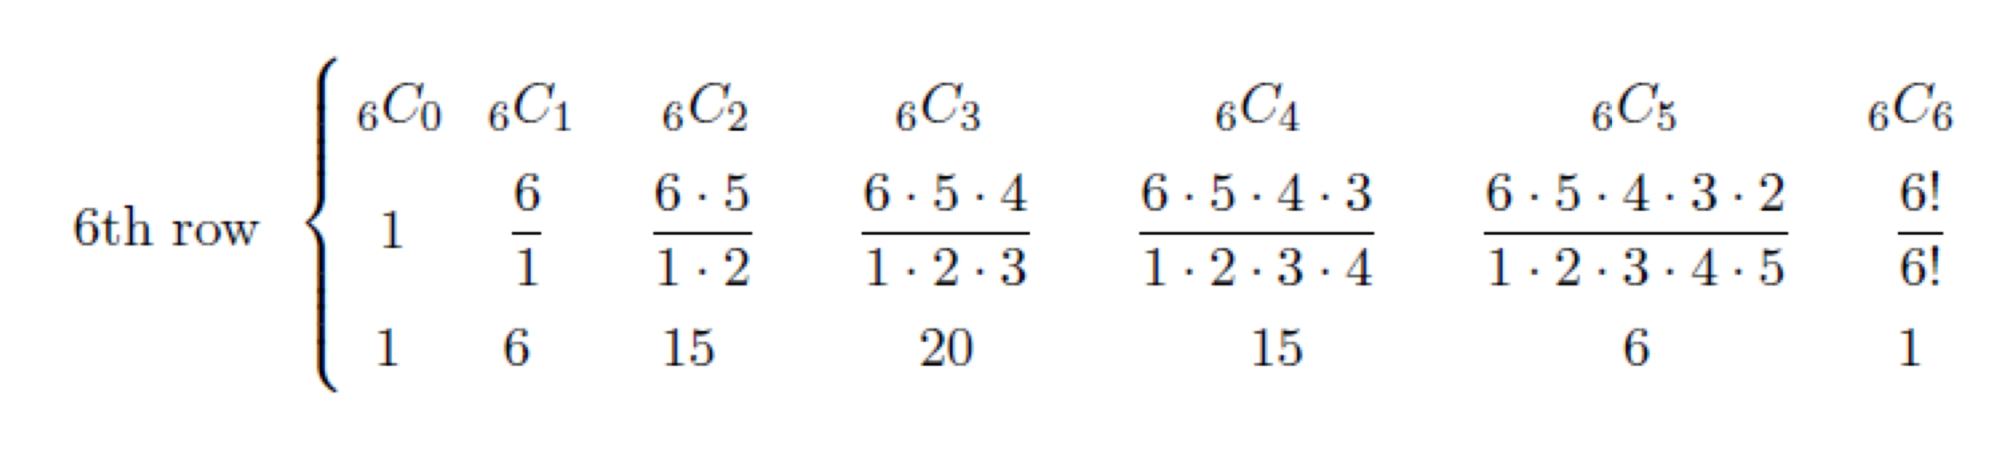
\includegraphics[width=0.6\linewidth]{./assets/binomialExpansion.png}
\end{center}

This theory is based on the Pascal's Triangle and the numbers of row $n$ correspond to the coefficients of each element of the expanded term.

We can calculate the coefficient of each part of the expanded term $k$ with combinatorics as follows: $\displaystyle {n\choose k}$

\begin{formula}[]{Binomial Expansion}
    \textbf{\textit{\underbar{In general:}}}
    \[
        (a + b)^n = 1a^nb^0 + {n\choose 1} a^{n-1}b^{1} + {n\choose 2} a^{n-2}b^{2} + \ldots + {n\choose n - 1} a^{1}b^{n - 1} + {n\choose n} a^{0}b^{n}
    \]
\end{formula}


\subsection{Overview}
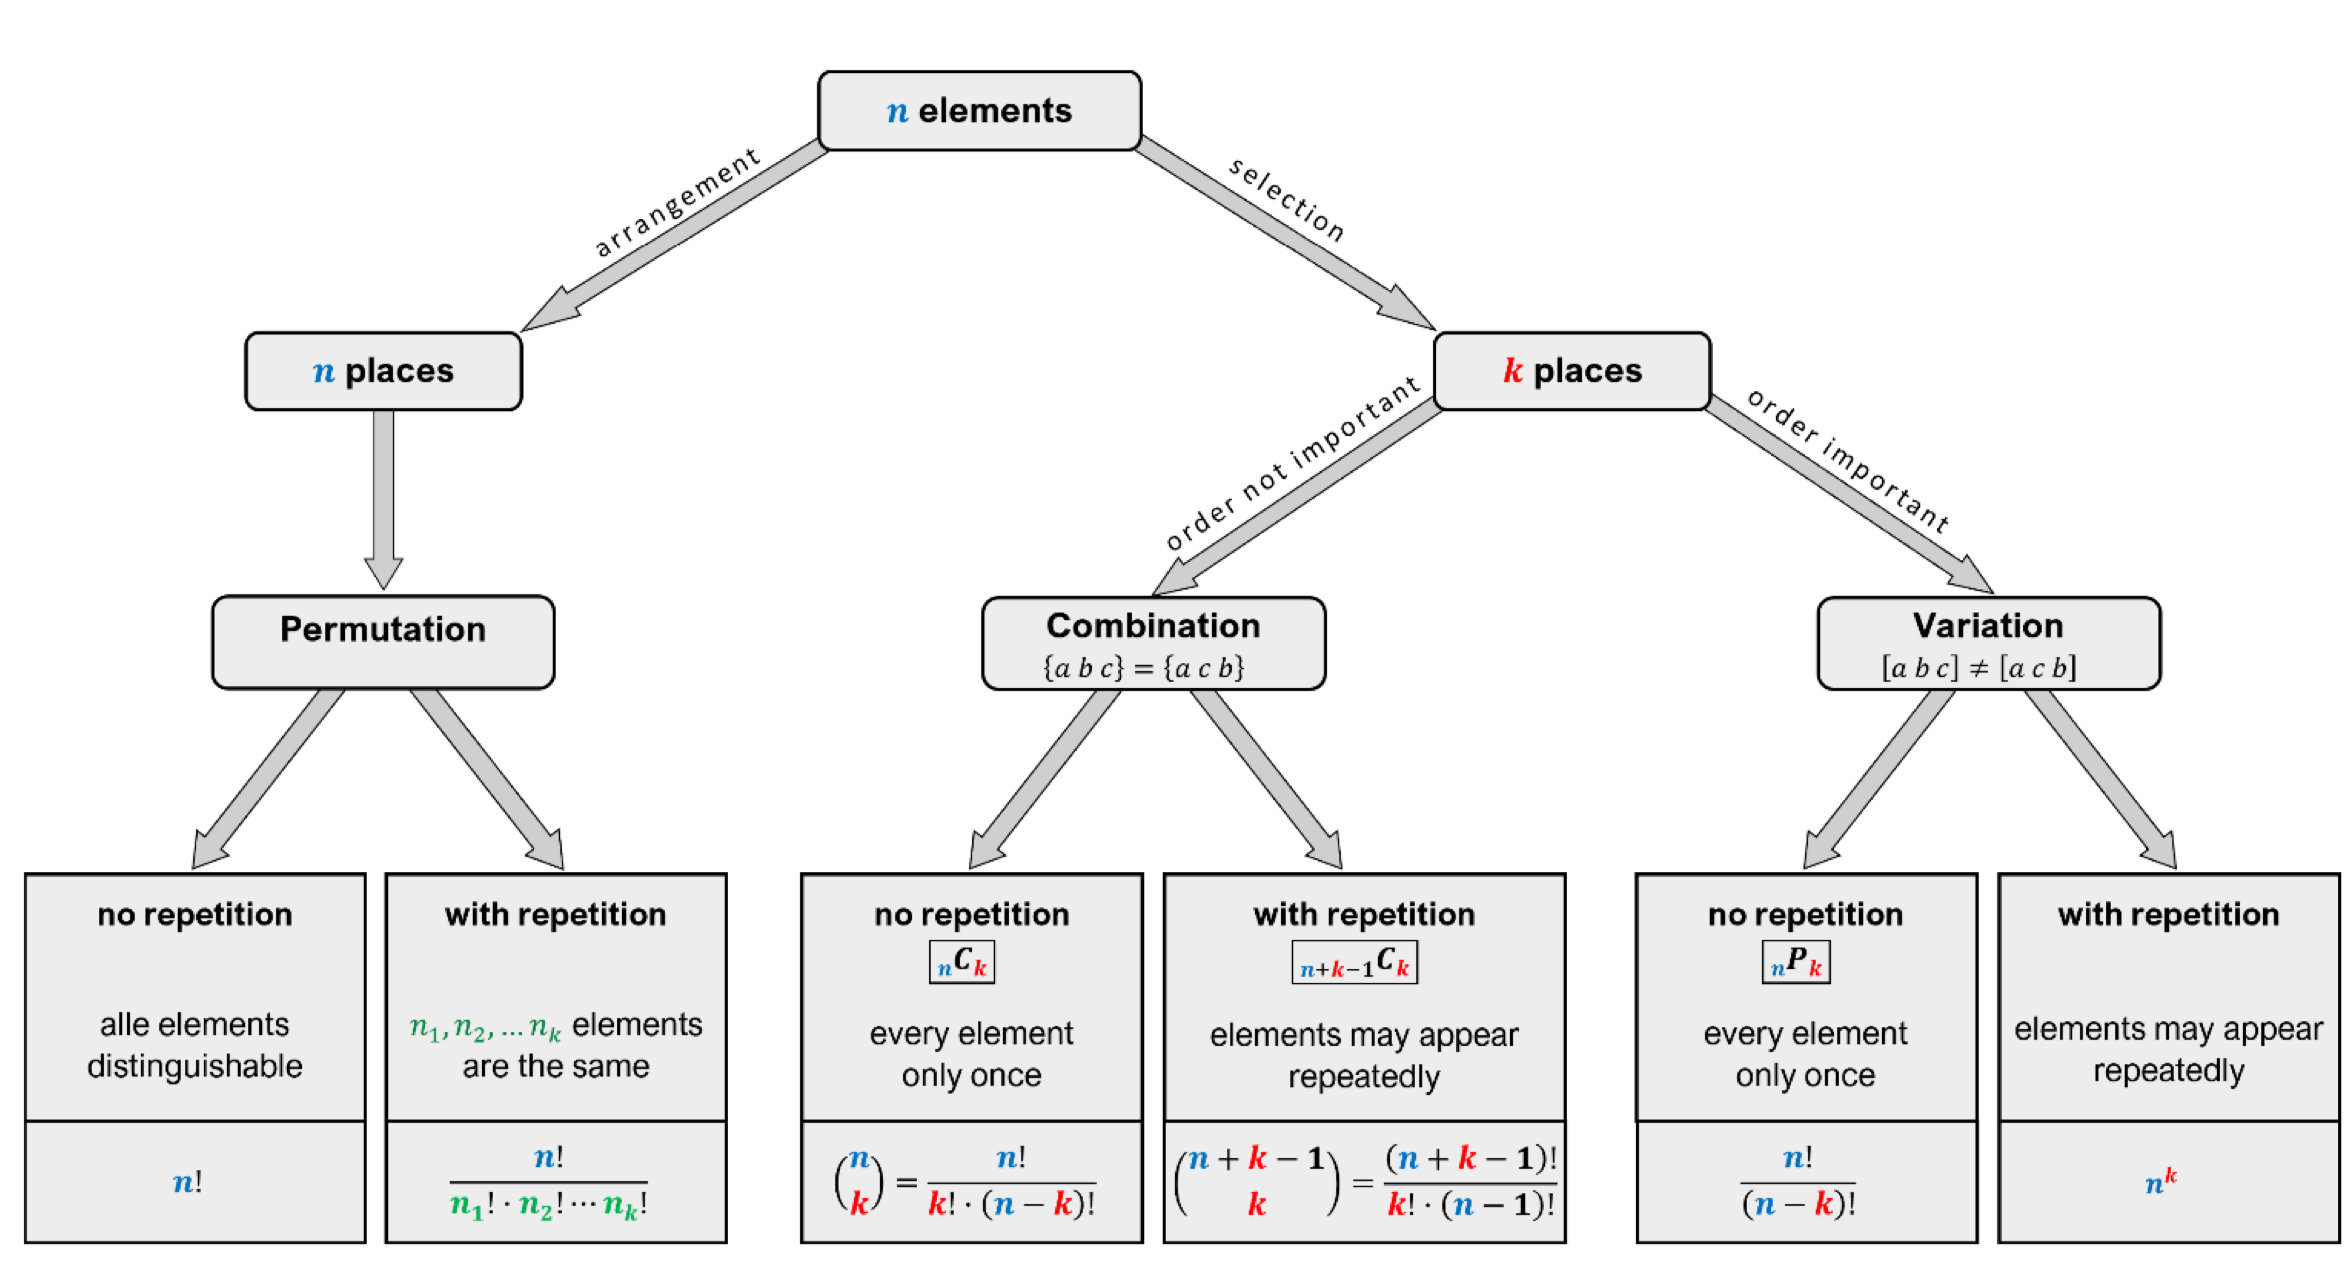
\includegraphics[width=1\linewidth]{./assets/overview.png}
